\documentclass[a4paper]{article}
\usepackage{amssymb}
\usepackage{graphicx}
\usepackage{hyperref}
\usepackage{microtype}

\title{H09M0A P\&D Embedded Systems and Multimedia}
\author{Seppe Iven - r0370830 \\ Koen Goetschalckx - r0375967}
\begin{document} 
\maketitle
\begin{center} Yu-Hui Huang, Johan Van Rompay, Hugo Van hamme
\end{center}

\section{Introduction}
This is an intermediate report about the MATLAB implementation of the P\&D assignment on subband coding, about the implementation of a speech codec. The main techniques used to create the codec are subband filtering and adaptive quantisation, with the goal of compressing a stereo audio signal. The MATLAB implementation uses fixed point numbers to mimic the working of a DSP. The parameters can be set in a flexible manner with the eye to optimal speech quality. \

This report first mentions the required specifications followed by the explanation of QMF filterbanks and adaptive differential quanisation. Next, this paper shows the general MATLAB structure of the implementation of the assignment and what all MATLAB scripts do. It then explains the criteria for the optimal values of the parameters, followed by some conclusions on the behaviour of those values. After this, the current set of optimal values is given. The final part of this paper is about the PESQ score for audio that has been encoded and decoded with this implementation and a general conclusion.

\section{Main design specifications}
The following list contains the specifications that the design of the codec has to meet.

\begin{itemize}
\item It accepts stereo signals
\item The sampling frequency is 8 kHz
\item The bitrate is 24 kbit/s per channel codec, with good to very good speech quality
\item The implementation consists of a QMF tree-structured filterbank with polyphase implementation
\item An adaptive differential quantisation scheme should be used for every subband signal
\item The filterbank of the codec consists of a minimum of 4 subbands
\item The total delay of the coder and decoder must not exceed a certain threshold: the entire one way communication delay (ADC, coding, encryption, decryption, decoding, DAC) should be less than 150ms. This puts a maximum on the number of subbands, on the complexity of the filters and on the buffer size in the cryptography section. Note that the encryption and decryption functionality is provided by another group and is not a part of this assignment.

\end{itemize}


\section{Splitting into subbands: QMF}
An input audio file is split into subbands by using a Quadrature Mirror Filter bank.
A QMF filter bank consists of a low-pass and high-pass filter $H_0(z)$ and $H_1(z)$, that split the audio file into a low-frequency and a high-frequency part. Such filter bank is used to efficiently create a two-way filter bank. A recursive implementation is used to split an audio file into four subbands. \\

QMF filters have some special properties:
\begin{itemize}
\item if $H_0(z)$ is a QMF filter, then $H_1(z) = H_0(-z)$ has the frequency response of $H_0$ mirrored around $\pi/2$.
\item if $H_0(z)$ is a QMF filter, then analysis filters $H_0(z)$ and $H_1(z) = H_0(-z)$ and synthesis filters $F_0(z)=H_1(-z)=H_0(z)$ and $F_1(z)=-H_0(-z) = -H_1(z)$ form an alias-free filter bank.
\end{itemize}

The second property indicates that a complete alias-free QMF filter bank can be defined by $H_0(z)$ alone. For the filter to be linear phase, this $H_0$ should be chosen symmetrical. Also, the filter should have an even amount of taps to avoid distortion at half the Nyquist frequency. \\

The first property indicates that if $H_0$ is a good low-pass filter, then $H_1$ is a good high-pass filter. \\

Given these properties and constraints, a simple polyphase implementation for a QMF filter bank can be designed, and is shown in figure \ref{fig:qmf}. The polyphase decomposition of $H_0(z)$ is:\\
\begin{center}
$H_0(z)$ = $E_0(z^2) + z^{-1} E_1(z^2)$ \\
\end{center}
From the first property, it follows that: \\
\begin{center}
$H_1(z)$ = $E_0(z^2) - z^{-1} E_1(z^2)$ \\
\end{center}
This leads to the efficient implementation of the filter bank shown in figure \ref{fig:qmf}.

\begin{figure}[hbt]
\includegraphics[width = \textwidth]{qmf}
\caption{Polyphase implementation of QMF filter bank}
\label{fig:qmf}
\end{figure}

\section{Adaptive differential quantisation and shizzle}
After filtering into subbands, the data is now encoded with an adaptive differential quantisation scheme. The quantizer can be seen in figure \ref{fig:quantization} and the dequantizer in figure \ref{fig:dequantization}. They contain the following signals:

\begin{itemize}
\item s(n) is the (serial) input signal
\item d(n) is the difference signal between the input signal and the prediction of the signal
\item z(n) is the quantized difference signal. This is also the output signal, hence the 'differential' in the name
\item d'(n) is the difference signal after quantization and dequantization. It thus resembles d(n) but is not exactly the same value
\item s'(n) is the sum of d'(n) and the prediction. It thus resembles s(n) but is not exactly the same value
\item s*(n) is the prediction of the next input signal 
\end{itemize}

As the name suggests, the stepsize is adaptive and based on the last values of d'(n) and a parameter $\phi$. The amount of values that influence the stepsize, is determined by a parameter 'buffer\_length'. Stepsize is calculated as follows:\\
$stepsize = round\_to\_zero(\phi*mean(abs(D'(n))))$
where D'(n) contains the last buffer\_length values of d'(n). The mean should be zero, so this equals to the first central moment. This is chosen instead of the variance for easy of calculation. \\
The reason of the use of d'(n) instead of d(n) is because the dequantizer only knows d'(n) and not d(n). For the same reason, the prediction is based on s'(n) and not in s(n). The prediction is a simple first order prediction, defined by the previous approximation of the signal s'(n) and a parameter $'\mu'$:\\
$s*(n) = \mu*s'(n-1)$.\\
The dequantizer can reconstruct s'(n) based on the z(n) it receives. It is thus lossy, since it cannot reconstruct the exact signal s(n). The benefit of this system is that only the transmitted signal is z(n), whose range is normally smaller than the range of s(n). Thus less bits are needed for encoding and transmitting z(n) than for s(n) and lossy compression is realized.
\begin{figure}[hbt]
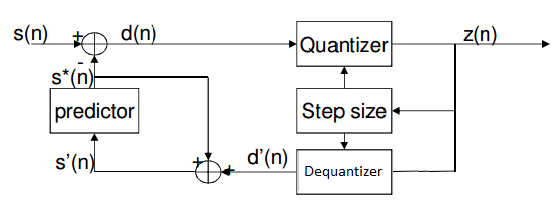
\includegraphics[width = \textwidth]{Quantization.png}
\caption{The Adaptive Differential Quantization scheme}
\label{fig:quantization}
\end{figure}
\begin{figure}[hbt]
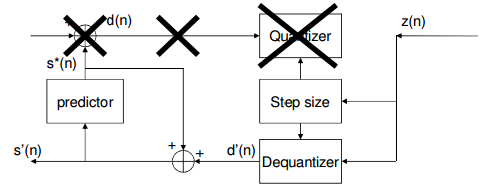
\includegraphics[width = \textwidth]{Dequantization.png}
\caption{The Adaptive Differential Dequantization scheme}
\label{fig:dequantization}
\end{figure}

Both the quantizer and dequantizer are initialised with the initial prediction $s*(0) = 0$ and the initial $stepsize(0) = 1$.

\section{MATLAB structure - Implementation overview}
This paper will now give a brief explanation of the MATLAB files that are used and their functionality.

TODO: Talk about all the scalings to make the numbers fit integers as much as possible etc

\subsection{generate\_some\_params.m}
This script can be run to generate the parameters that are used to call run.m

\subsection{run.m}
This is the main function that is used to divide an audio file into subbands, encode and decode those subbands, and synthesize them again to create an audio signal that closely resembles the original signal. Accepted audio files are .wav-files that are stereo or pairwise mono. The wanted input audio file for this should be named 'input.wav'.
\\
The input is scaled to a 16 bit signed integer. The input is then split into subbands by calling analysis.m. These subbands are first encoded by calling encoded.m. The result is what would be transmitted or saved in real use. Next, the function decodes the result by calling decode.m. Finally, the subbands are recombined by calling synthesis.m and the PESQ score for the reconstructed audio file is calculated. For this calculation, only one channel is considered, because in most of the test files the two channels are the same (effectively mono). Even when this is not the case, a noticeable increase of score in one channel should lead to a similar increase in the other for real life signals.

\subsection{analysis.m}
This MATLAB function mainly splits the stereo (or pairwise mono) channels into separate channels, and feeds splits them into subbands by calling get\_subbands.m.

\subsection{get\_subbands.m}
This function recursively splits an audio channel into its subbands. It does this by applying polyphase QMF filters, as explained earlier in this paper. These filters are generated with a script that was given as as part of the assignment and defined by its parameters.
Convolutions are used to apply the filters. Since this is a sum of products, the output values exceed the 16-bit range. The output is thus downscaled again. This downscaling is done by division of a power of two, so it is easily implementable as a bitshift. The exponent of two can be chosen, as it is a parameter. This gives rise to a trade-off between clipping and quantisation noise. A too small exponent leads to the former, while a too large exponent leads to relatively larger quantisation noise.

\subsection{encode.m}
This function uses an adaptive differential quantisation method to compress an input signal. Such method is covered in an earlier part of this paper. A parameter determines the maximum output and thereby the amount of bits needed. Larger values are clipped, which should be avoided. For analysis purposes, the function keeps track of the number of times this happened.

\subsection{decode.m}
This function is the inverse of encode.m: it takes the output of the adaptive differential quantisation function and constructs s'(n), which approximates the original input signal s(n).

\subsection{synthesis.m}
This function is the inverse of get\_subbands.m: its input are the separate subbands and it combines (synthesises) back into one signal. The filters used for this are the same QMF filters used for analysis, as explained earlier in the text.

\section{Criterion for optimal values}
From p127, we got the values for phi TODO we assumed gaussian distribution
Optimal values also includes: filter lengths etc just put here as many parameters as possible i guess
From the book: mu is fixed per fequency band. Estimate it such that the energy of the prediction error s(n) - mu*s(n-1) is minimized

\section{General findings on the behaviour of PESQ}
Don' really know what to put here but the assignment said we need this section. Maybe this is an introduction/conclusion section?

\section{Set of optimal values of controllable parameters}
TODO hier onze finale waarden ingeven en zeggen hoe we eraan komen (zie boek: sommige vanuit theorie, sommigen bruteforce)
TODO also zeggen dat we optimised hebben voor de combined shizzle omdat die ons beter lijkt dan voor één aparte; dan zeggen wat de optimale en de minst optimale PESQ waarden zijn bij de verschillende .wav bestandjes
TODO zeggen dat deze waarden subject to change zijn en mogelijk niet onze finale waarden

NOW NAME ALL PARAMETETERS! AND WRITE ABOUT MOTIVATION TO CHOOSE THEM! This includes:
Amount of subbands
Truncating vs rounding
Scalings

This section will handle all of the parameters that define the implementation of the speech codec. Please note that although these values are currently our optimal values, they may be subject to changes in the future. For example, a quantization method was recently changed from rounding to rounding towards zero, to better comply with rounding in C. This all may influence the optimal values of the parameters.

The QMF filters that are generated with the given function QMF_design.m are characterized by the following parameters:

\begin{itemize}
\item The sampling frequency, which is mandatory 8 kHz
\item The total transition width of the prototype filter. This is default at fs/10, and thus we have left it at 800
\item The minimum stopband attenuation of the prototype filter, which we have left at the default value of 60 dB
\item The frequency step for finding the optimal cut-off frequency, which we have left at the default value of 10
\item The maximum number of iterations, which we have at 600
\item The filter lengths, which we have at 64 for the filter at the first depth and 32 for the filters at the second depth. We have chosen these lengths as a compromise between filter quality and implementation delay
\end{itemize}

The values of $\mu$, used in the prediction of the next signal, are different for each subband. TODO hoe gevonden, patterns erin? Also in welke scaling weergeven? $*2^15$ of niet?

The values of $\phi$, used in the calculation of the stepsize, are different for each subband. TODO hoe gevonden, patterns erin? Also in welke scaling weergeven? $*2^15$ of niet? TODO gestart vanuit paper

The number of bits per sample is also different for each subband. Lower subbands have more bits per sample, since they are more important to the human hearing. The lowest to highest subbands have 5, 4, 3 and 0 bits per sample respectively. Note that the highest subband is simply thrown away.

The parameter buffer_lengths, used in the calculation of the stepsize, is equal to 10 for every subband.

For the values of $\phi$, we started from the theory TODO reference. From there, all values of $\phi$, $\mu$ and buffer_lengths TODO also scalings were finetuned by trial and error: changing values, watching and following trends.

\section{Delay of the implementation}
Delay due to: 
Filtering/convolving (filter length and time to execute this (=1?))
Quantization
Dequantization
Filtering/convolving

\section{Final SNR \& PESQ}
TODO zeggen dat we SNR niet hebben gebruikt en daar een reden voor verzinnen bv PESQ is beter

\section{Conclusion}
TODO spekken (zie taalgebruik van bossie) over alle secties die we behandeld hebben in deze paper
TODO zeggen dat we een goede maar niet finale MATLAB implementatie hebben (bv de deling die we nog aangepast hebben om op C te lijken; alsook dat onze final parameters nog niet final zijn maar subject to optimization)

\section{References}
\begin{itemize}
\item S. K. Agrawal and O. P. Sahu, Two-Channel Quadrature Mirror Filter Bank: An Overview, 23/03/2016, \url{http://www.hindawi.com/journals/isrn/2013/815619/}
\end{itemize}
\end{document}

TODO scan for codex instead of codec
TODO include total delay of code/encode: should be less than 150ms
TODO rechterdeel in run
TODO iets over delay?